\documentclass{article}
\usepackage{tikz}

\begin{document}
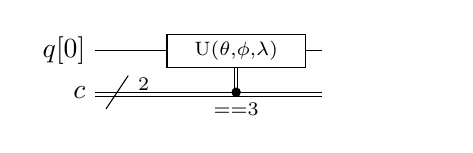
\begin{tikzpicture}[scale=1.000000,x=1pt,y=1pt]
\filldraw[color=white] (0.000000, -7.500000) rectangle (82.000000, 22.500000);
% Drawing wires
% Line 1: q0 W q[0]
\draw[color=black] (0.000000,15.000000) -- (82.000000,15.000000);
\draw[color=black] (0.000000,15.000000) node[left] {$q[0]$};
% Line 2: c W c
\draw[color=black] (0.000000,0.000000) -- (82.000000,0.000000);
\draw[color=black] (0.000000,0.000000) node[left] {$c$};
% Done with wires; drawing gates
% Line 3: c / 2 %% ==3
\draw (51.000000, -.500000) node[text width=144pt,below,text centered]{\scriptsize ==3};
%\draw (6.000000, -6.000000) -- (14.000000, 6.000000);
\draw (12.000000, 3.000000) node[right] {$\scriptstyle{2}$};
% Line 4: q0 G {u($\theta$,$\phi$,$\lambda$)} c  width=50
\draw (50.5000000,15.000000) -- (50.5000000,0.000000);
\draw (51.5000000,15.000000) -- (51.5000000,0.000000);
\begin{scope}
\draw[fill=white] (51.000000, 15.000000) +(-45.000000:35.355339pt and 8.485281pt) -- +(45.000000:35.355339pt and 8.485281pt) -- +(135.000000:35.355339pt and 8.485281pt) -- +(225.000000:35.355339pt and 8.485281pt) -- cycle;
\clip (51.000000, 15.000000) +(-45.000000:35.355339pt and 8.485281pt) -- +(45.000000:35.355339pt and 8.485281pt) -- +(135.000000:35.355339pt and 8.485281pt) -- +(225.000000:35.355339pt and 8.485281pt) -- cycle;
\draw (51.000000, 15.000000) node {\scriptsize {U($\theta$,$\phi$,$\lambda$)}};
\end{scope}
\filldraw (51.000000, 0.000000) circle(1.500000pt);
\draw[color=black] (0.000000,-1.5000000) -- (82.000000,-1.5000000);
\draw (4.000000, -6.000000) -- (12.000000, 6.000000);
% Done with gates; drawing ending labels
% Done with ending labels; drawing cut lines and comments
% Done with comments
\end{tikzpicture}
\end{document}
